\subsection{Software}
Im folgenden wird die Ansteuerung und Auswertung der elektrischen Komponenten näher beschrieben. Außerdem wird die Kommunikation zwischen der Host- und Target-Plattform erläutert. Als Zielplattform wird ein \ac{BBB} verwendet, auf welchem eine Linux-Distribution ausgeführt wird. In der folgenden Abbildung sind die einzelnen Bausteine und deren Verbindung zu der Zielplattform dargestellt.

\begin{figure}[!h]
\centering
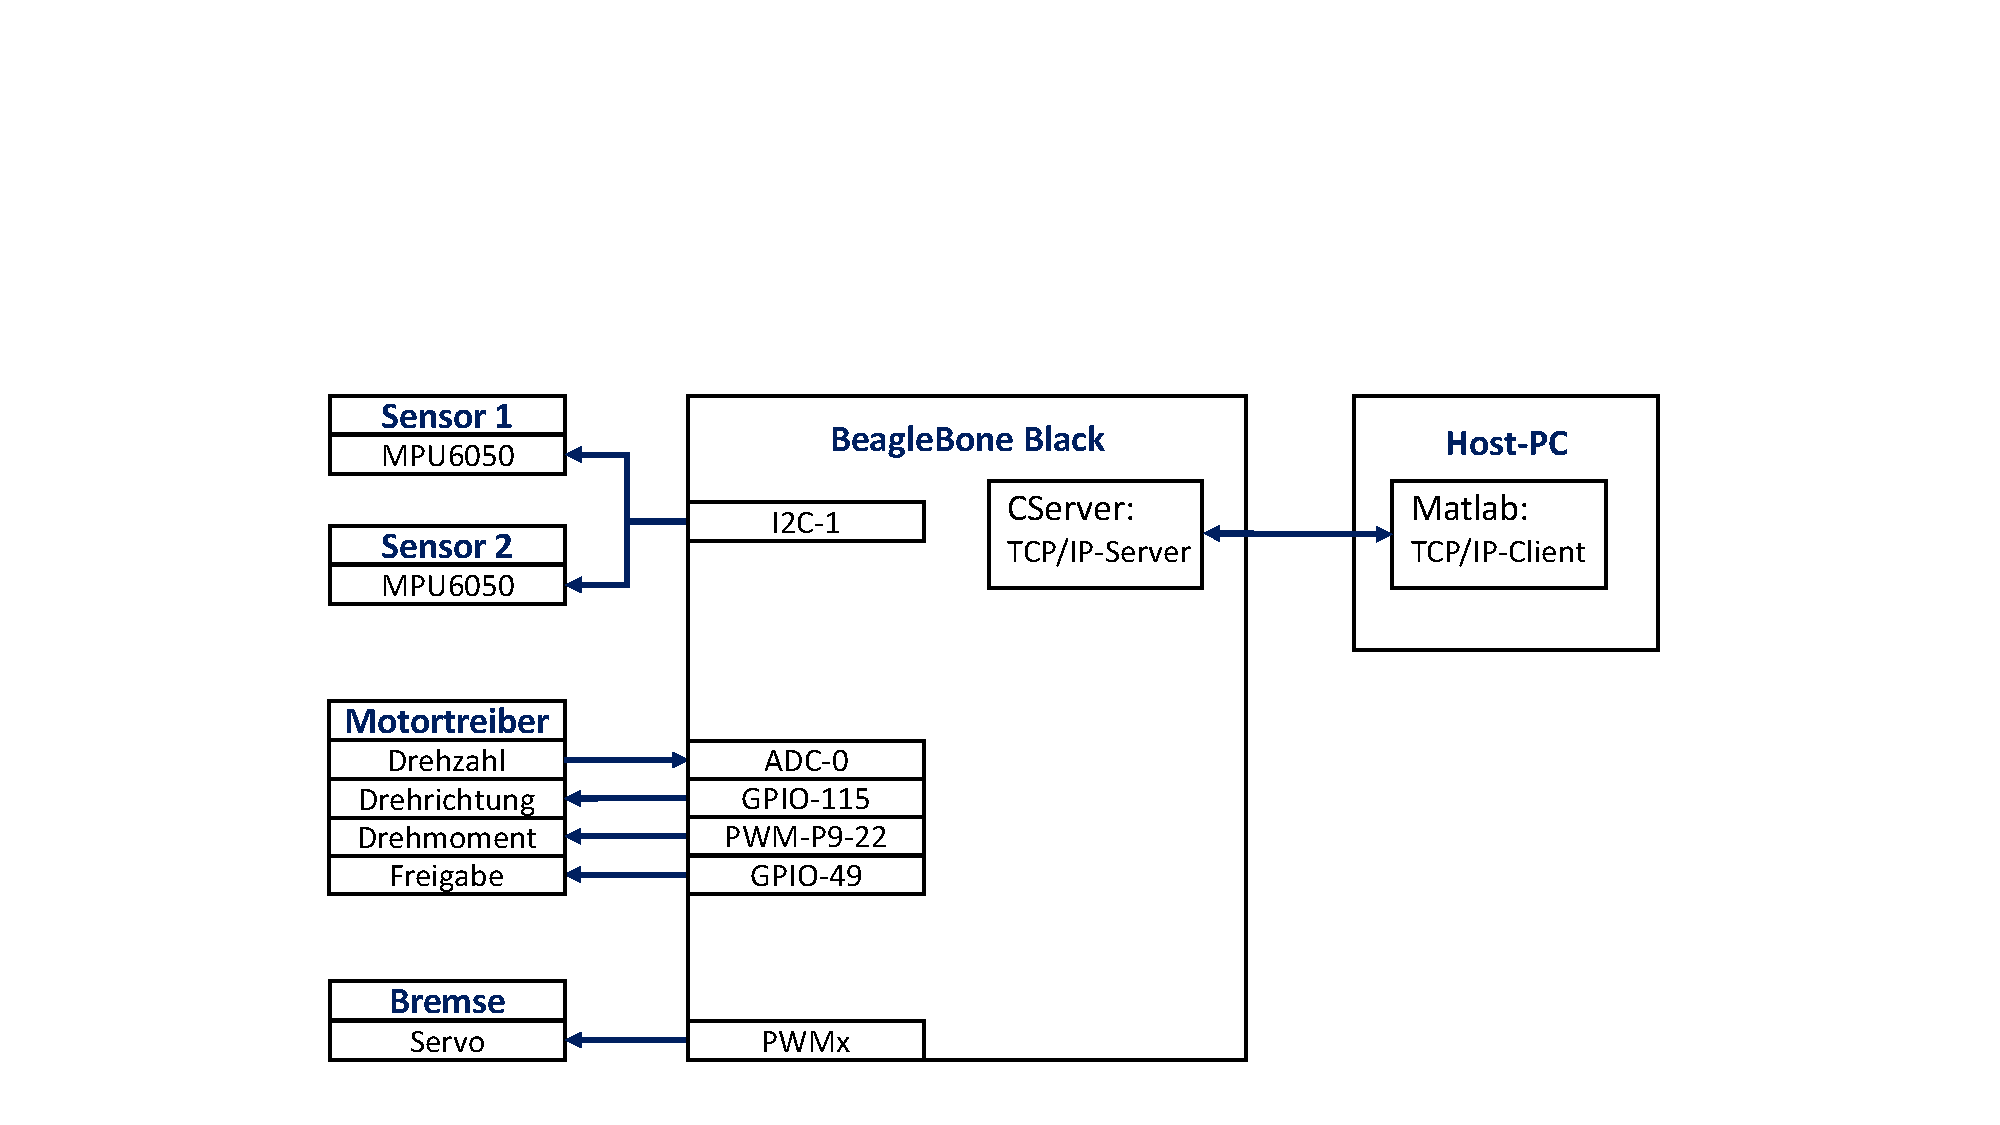
\includegraphics[width=0.8\linewidth, trim={4cm 1cm 5cm 6cm},clip]{img/ElekAufbau_Kommunikation}
\caption{Blockschaltbild der Komponenten, Quelle: eigene Darstellung}
\end{figure}

Um die verschiedenen Versuche und Messungen durchzuführen wird eine Software-Basis entworfen, welche als Grundlage für die verschiedenen Applikationen dient. Diese Grundlage umfasst eine objektorientierte Kapselung der Hardware, die TCP-Server-Implementierung um mit der MATLAB-Anwendung zu kommunizieren, die Definition zweier Komponenten, welche als separate Tasks ausgeführt werden und eine Kommunikationsstruktur für den Datenaustausch. Der Aufbau dieser Bausteine wird in den folgenden Abschnitten näher erläutert.

\subsubsection{Hardware-Schnittstelle}
Die Interaktion mit den Treibern des Betriebssystems wird mit Hilfe von Klassen gekapselt. Dadurch entsteht eine einheitliche und benutzerfreundliche Schnittstelle zwischen Hard- und Software. (Interface-Darstellen, ansonsten kommt das von Christian, haben wir also nicht viel zu erklären (Im Vorwort darauf verweisen was wir nicht selber gemacht haben)).

Interface-Listing

\subsubsection{TCP/IP-Verbindung}
Die Kommunikation zwischen der \ac{BBB}- und der MATLAB-Applikation verläuft über eine TCP/IP-Verbindung. Hierfür wird auf dem \ac{BBB} ein Server ausgeführt, welcher auf die Verbindungsanfrage des MATLAB-Clients wartet. Die Vorteile des gewählten Protokolls liegen einerseits in der gesicherten und abstrahierten Datenübertragung, andererseits in den anwendungsfreundlichen Bibliotheken für Linux und MATLAB. Mit Hilfe einer simulierten Ethernet-Verbindung über USB wird ein privates Netzwerk zwischen der Zielplattform und dem Entwiclungs-PC 

Bild mit Adressen/Socket, etc.

\subsubsection{Komponentenarchitektur}
Server/Comm-Componenten, Control-Componente (kriegt die ne FSM für die verschiedenen Versuche? ist zwar schöner aber auch bisschen over-the-top)

\subsubsubsection{Kommunikation mittels Nachrichten}
Die Kommunikation der beiden Prozess auf dem \ac{BBB} erfolgt mit Hilfe von Nachrichten. Dieser werden mit Hilfe von Queues, welche im \ac{SHM} angelegt werden, zwischen den beiden Prozessen ausgetauscht. Zusätzlich wird dieselbe Nachrichtenstruktur verwendet um Daten zwischen dem \ac{BBB} und der MATLAB-Anwendung auszutauschen. Hierfür werden die Daten als Byte-Stream über die TCP/IP-Verbindung übertragen. 

\begin{figure}[!h]
\centering
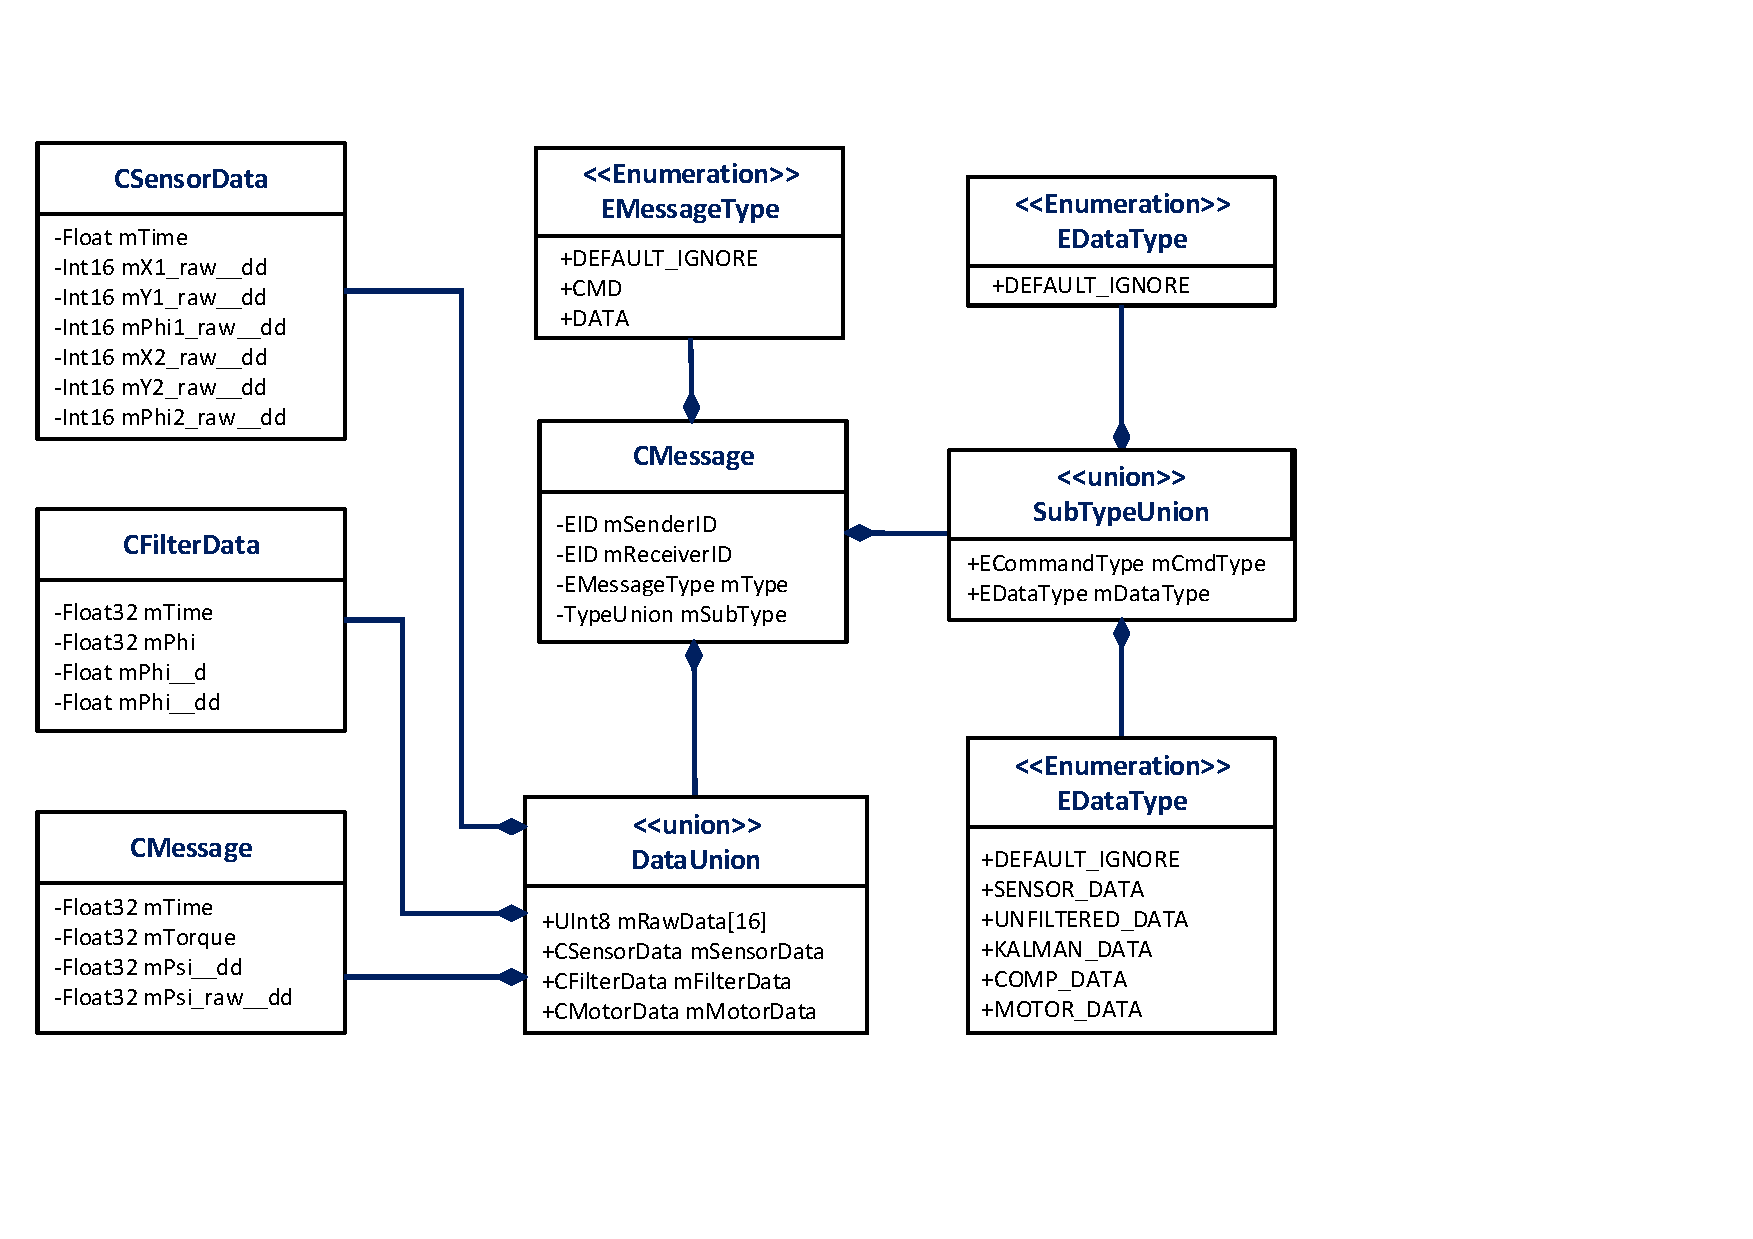
\includegraphics[width=0.8\linewidth, trim={0cm 2cm 7cm 2cm},clip]{img/UML_MessageClassDiag}
\caption{UML Nachrichtenaufbau, Quelle: eigene Darstellung}
\end{figure}

Die Nachrichten bestehen aus einem Header, welcher allgemeine Informationen wie Sender, Empfänger und den Nachrichtentyp enthält. Grundsätzlich wird zwischen Nachrichten zur Übertragung von Befehlen und Daten unterschieden (Schachetln weglassen, es gibt nur einen Nachrichtentyp, --> Typ wird zu Event/Kommando und es gibt ein TransmitData-Event, im jetzten TypeUnion Byte wird in dem Fall spezifziert um welche Daten es sich handelt.)

Das Datenfeld wird genutzt um relevante Informationen wie Sensor-, Filter- und Motorwerte an die MATLAB-Applikation zu übermitteln.